\subsection{Parallel Ports}
There are several parallel ports implemented in the FPGA that support input, output, and
bidirectional transfers of data between the \processor~processor and I/O peripherals. As 
illustrated in Figure~\ref{fig:parallel_port}, each parallel port is assigned a {\it Base}
address and contains up to four 32-bit registers. Ports that have output capability include a
writable {\it Data} register, and ports with input capability have a readable {\it
Data} register. Bidirectional parallel ports also include a {\it Direction} register that 
has the same bit-width as the {\it Data} register. Each bit in the {\it Data} register can be
configured as an input by setting the corresponding bit in the {\it Direction} register to 0,
or as an output by setting this bit position to~1. The {\it Direction} register is assigned the
address {\it Base} + 4.

\begin{figure}[h!]
   \begin{center}
       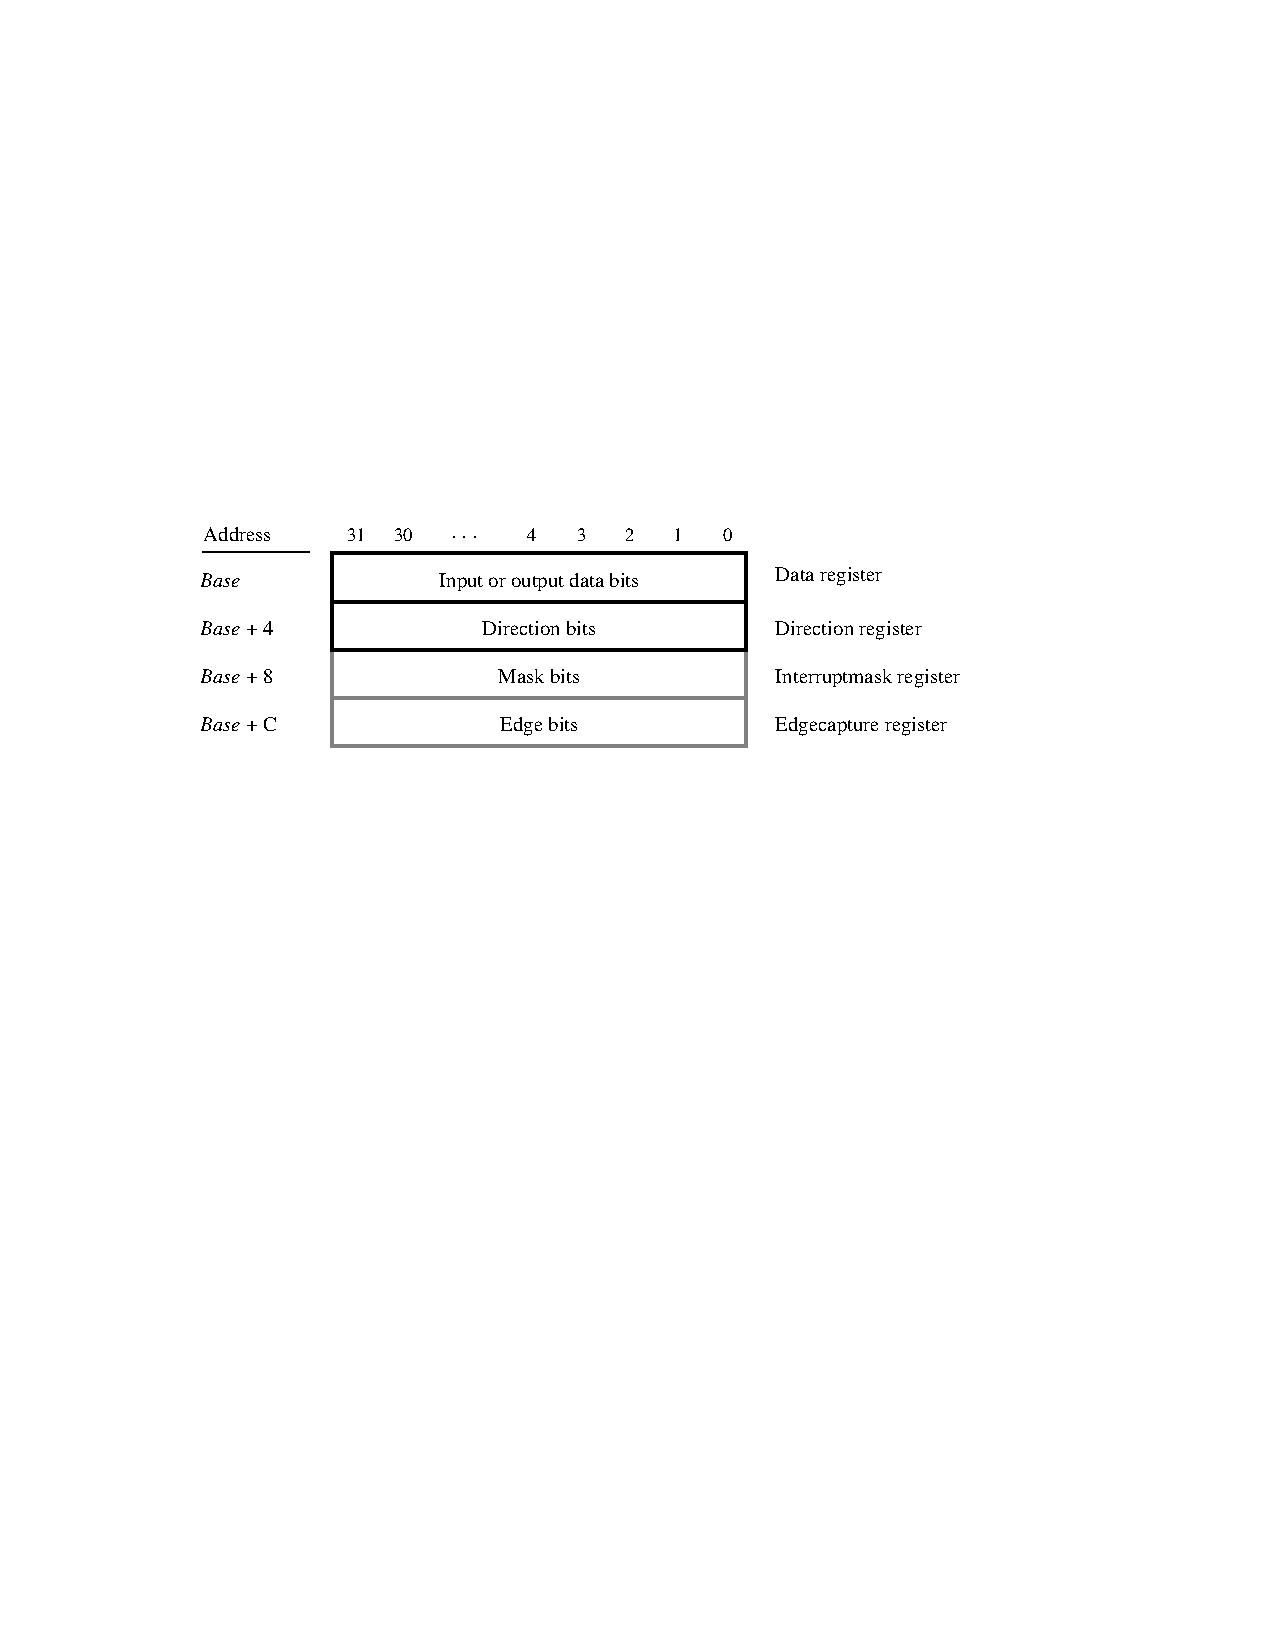
\includegraphics{../../../common/figs/FPGA_PP.pdf}
   \end{center}
   \caption{Parallel port registers in the {\it \systemNameFull}.}
	\label{fig:parallel_port}
\end{figure}

Some of the parallel ports have registers at addresses 
{\it Base} + 8 and {\it Base} + C, as indicated in Figure~\ref{fig:parallel_port}. These
registers are discussed in Section \ref{sec:exceptions}.


